\documentclass[11pt]{article}


\usepackage[margin=1in,a4paper]{geometry}
\usepackage[utf8]{inputenc}
\usepackage[T1]{fontenc}
\usepackage{lmodern}
\usepackage{tabularx}
\usepackage{quoting}
\usepackage{fancyhdr}
\usepackage{graphicx}
\usepackage{nicefrac}
\usepackage{sectsty}
\usepackage{graphicx}
\usepackage[T1]{fontenc}
\usepackage{epigraph} %quotes
\usepackage{amssymb} %math symbols
\usepackage{mathtools} %more math stuff
\usepackage{amsthm} %theorems, proofs and lemmas
\usepackage{optidef} %fast optimization problem notation
\usepackage{changepage}
\usepackage{gensymb}
\usepackage[ruled,vlined,noend,linesnumbered]{algorithm2e} %algoritms/pseudocode


\usepackage{biblatex}

%% asmthm notation
\newtheorem{theorem}{Theorem}[section]
\newtheorem{corollary}{Corollary}[theorem]
\newtheorem{lemma}[theorem]{Lemma}
\newtheorem{problem}{Problem}
\newtheorem{definition}{Definition}
\newtheorem{claim}{Claim}[section]


%% declaring abs so that it works nicely
\DeclarePairedDelimiter\abs{\lvert}{\rvert}%
\DeclarePairedDelimiter\norm{\lVert}{\rVert}%

\let\oldnl\nl% Store \nl in \oldnl
\newcommand{\nonl}{\renewcommand{\nl}{\let\nl\oldnl}}% Remove line number for one specific line in algorithm

\title{BIOENG-404 - Homework 4: SCONE}
\author{
    Titouan Renard
    - MT : Robotics 
}
\date{\today}



\begin{document}


\maketitle

\section{Healthy Gait}

The solution provided by the optimization process (which converges relatively fast) is quite good. The gait appears natural when played as a video but a close examination of the gait parameters (pelvic tilt, hip, knee and ankle flexion as well as ground reaction forces, displayed in figure \ref{healthy_gait}) show that the model gives results slightly off compared to measured data in humans. The curves have the approximate shape of the real-life data but their amplitude and timing is slightly off. Furthermore one observes that the ankle flexion displays a dip in angle at $\sim 25\%$ of the gait cycle that simply doesn't exist in humans. This model seems more useful as a toy-model, to rapidly test out hypotheses rather than as an accurate prediction tool (as is often the case when modeling complex dynamical systems). The render allows for the observation of gait kinematics as displayed in figure \ref{healthy_render}.

\begin{figure}[h!]
    \centering
    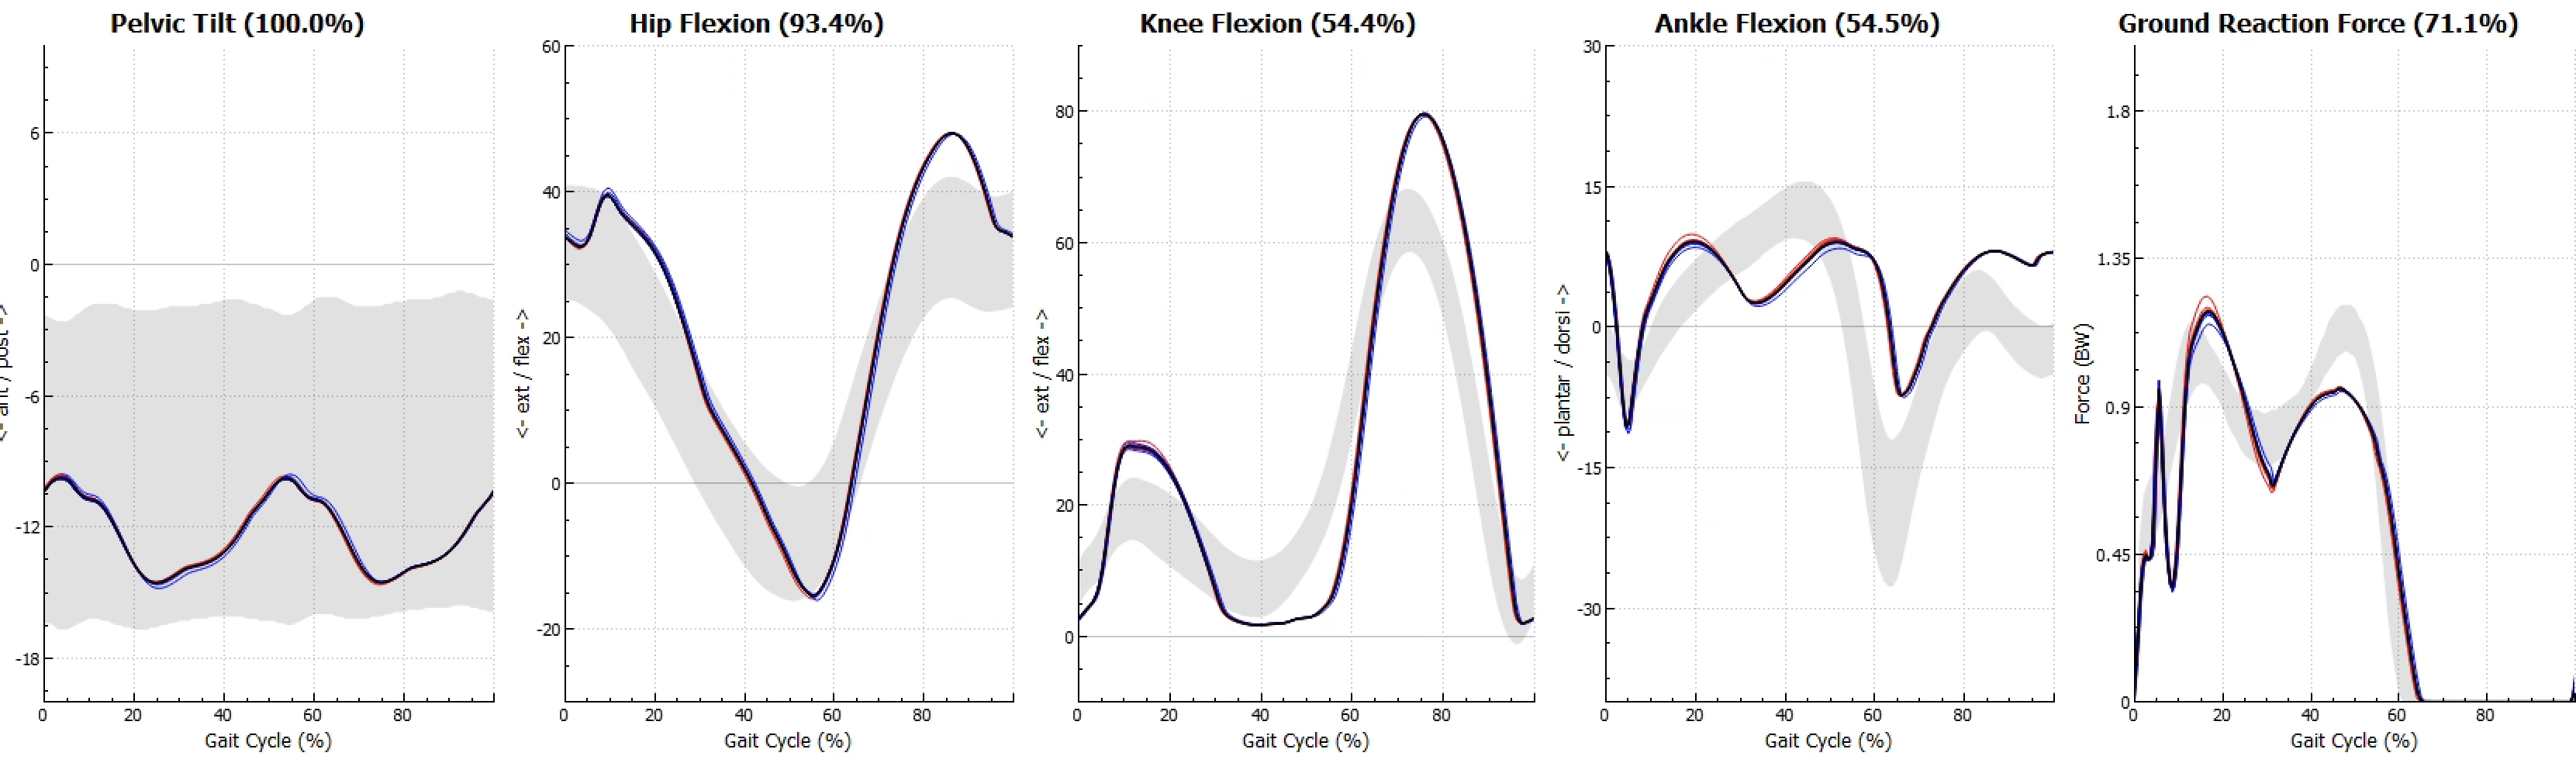
\includegraphics[width=0.9\textwidth]{screens/healthy_gait.png}
    \caption{Gait parameters as observed in the SCONE simulation of the gait of a healthy subject. The grayed-out area show distribution of gait parameters in healthy humans, the colored lines show the gait parameter evolution over multiple gait cycle for our optimal solution.}
    \label{healthy_gait}
\end{figure}

\begin{figure}[h!]
    \centering
    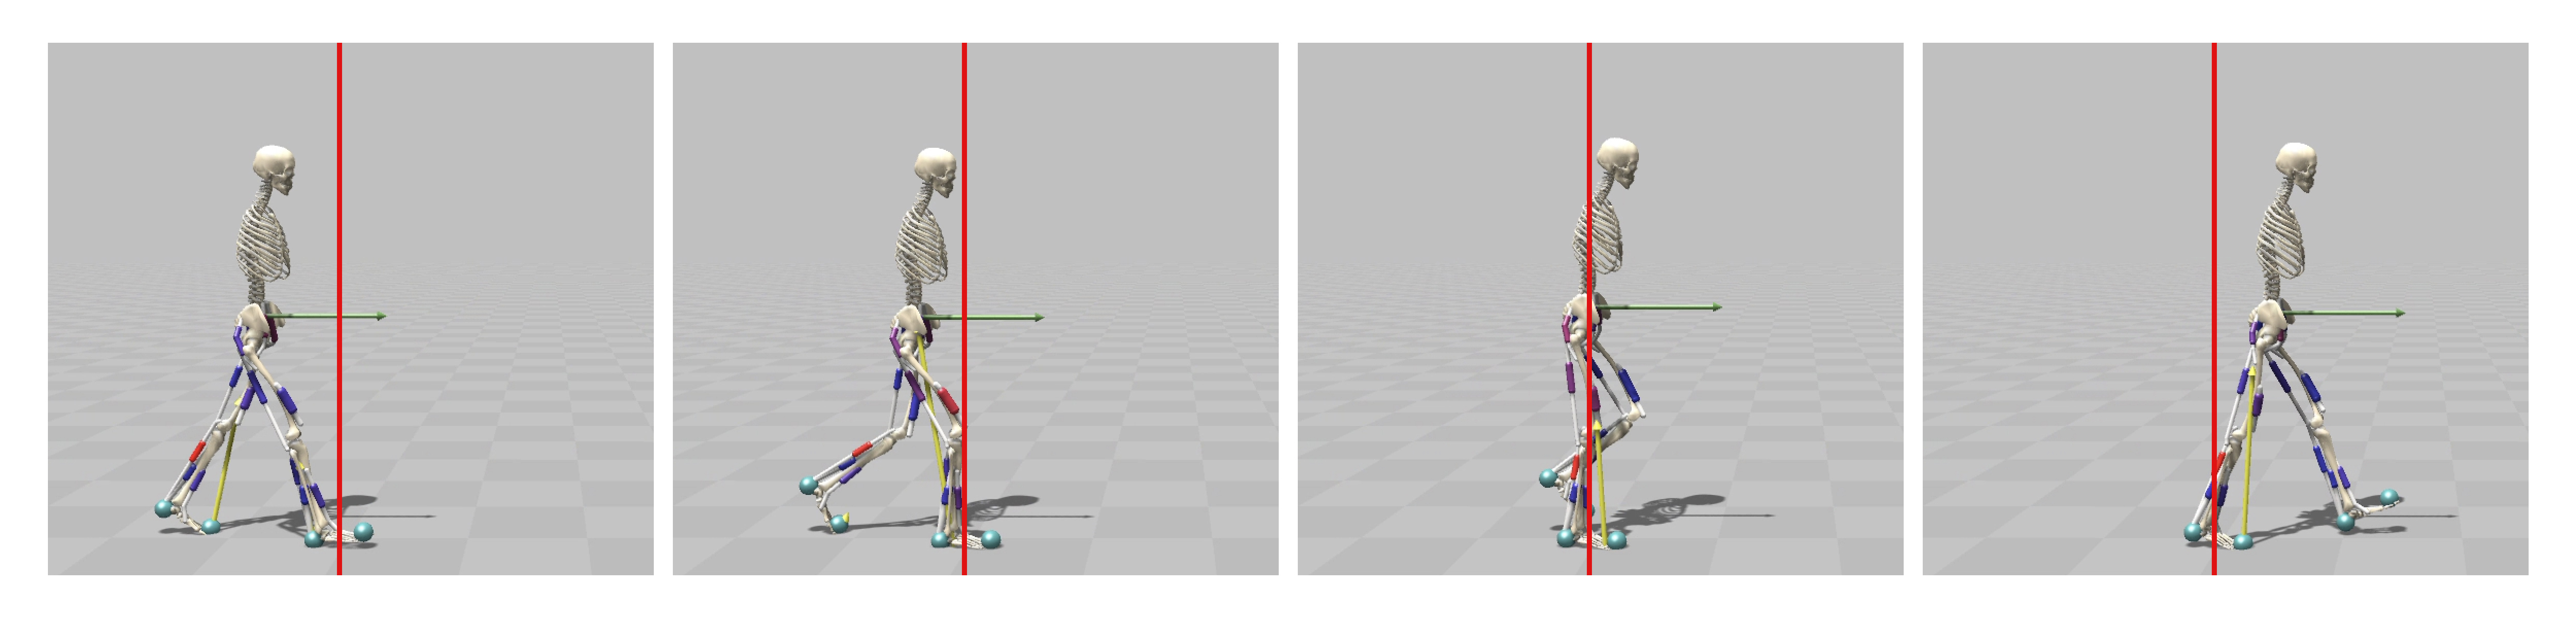
\includegraphics[width=\textwidth]{screens/healthy_render.jpg}
    \caption{Rendering of the optimization solution produced by the healthy model and controller. The stills are presented in chronological order from left to right. T red line denotes a reference point in space between the different stills. One can clearly observe heel contact (on the leftmost still), a foot-flat phase (on the two centered stills) and then toe-off (on the rightmost still).}
    \label{healthy_render}
\end{figure}

\section{Pathological Gait : Plantarflexor Muscle Atrophy}

We reduce the maximum force that can be produced by the plantarflexor muscles (\textit{gastrocnemius} and \textit{soleus}). The principal kinetic adaptation is (quite obviously) a reduction of the amplitude of plantarflexion as is clearly visible on the ankle figure plot of the gait analysis in figure \ref{atrophic_gait}. A more general observation is that the gait analysis signal is generally more noisy as it seems this system is harder to control by the control architecture in our model. The speed of walking is also slower (we relaxed the speed constraint before launching the optimization process).

\begin{figure}[h!]
    \centering
    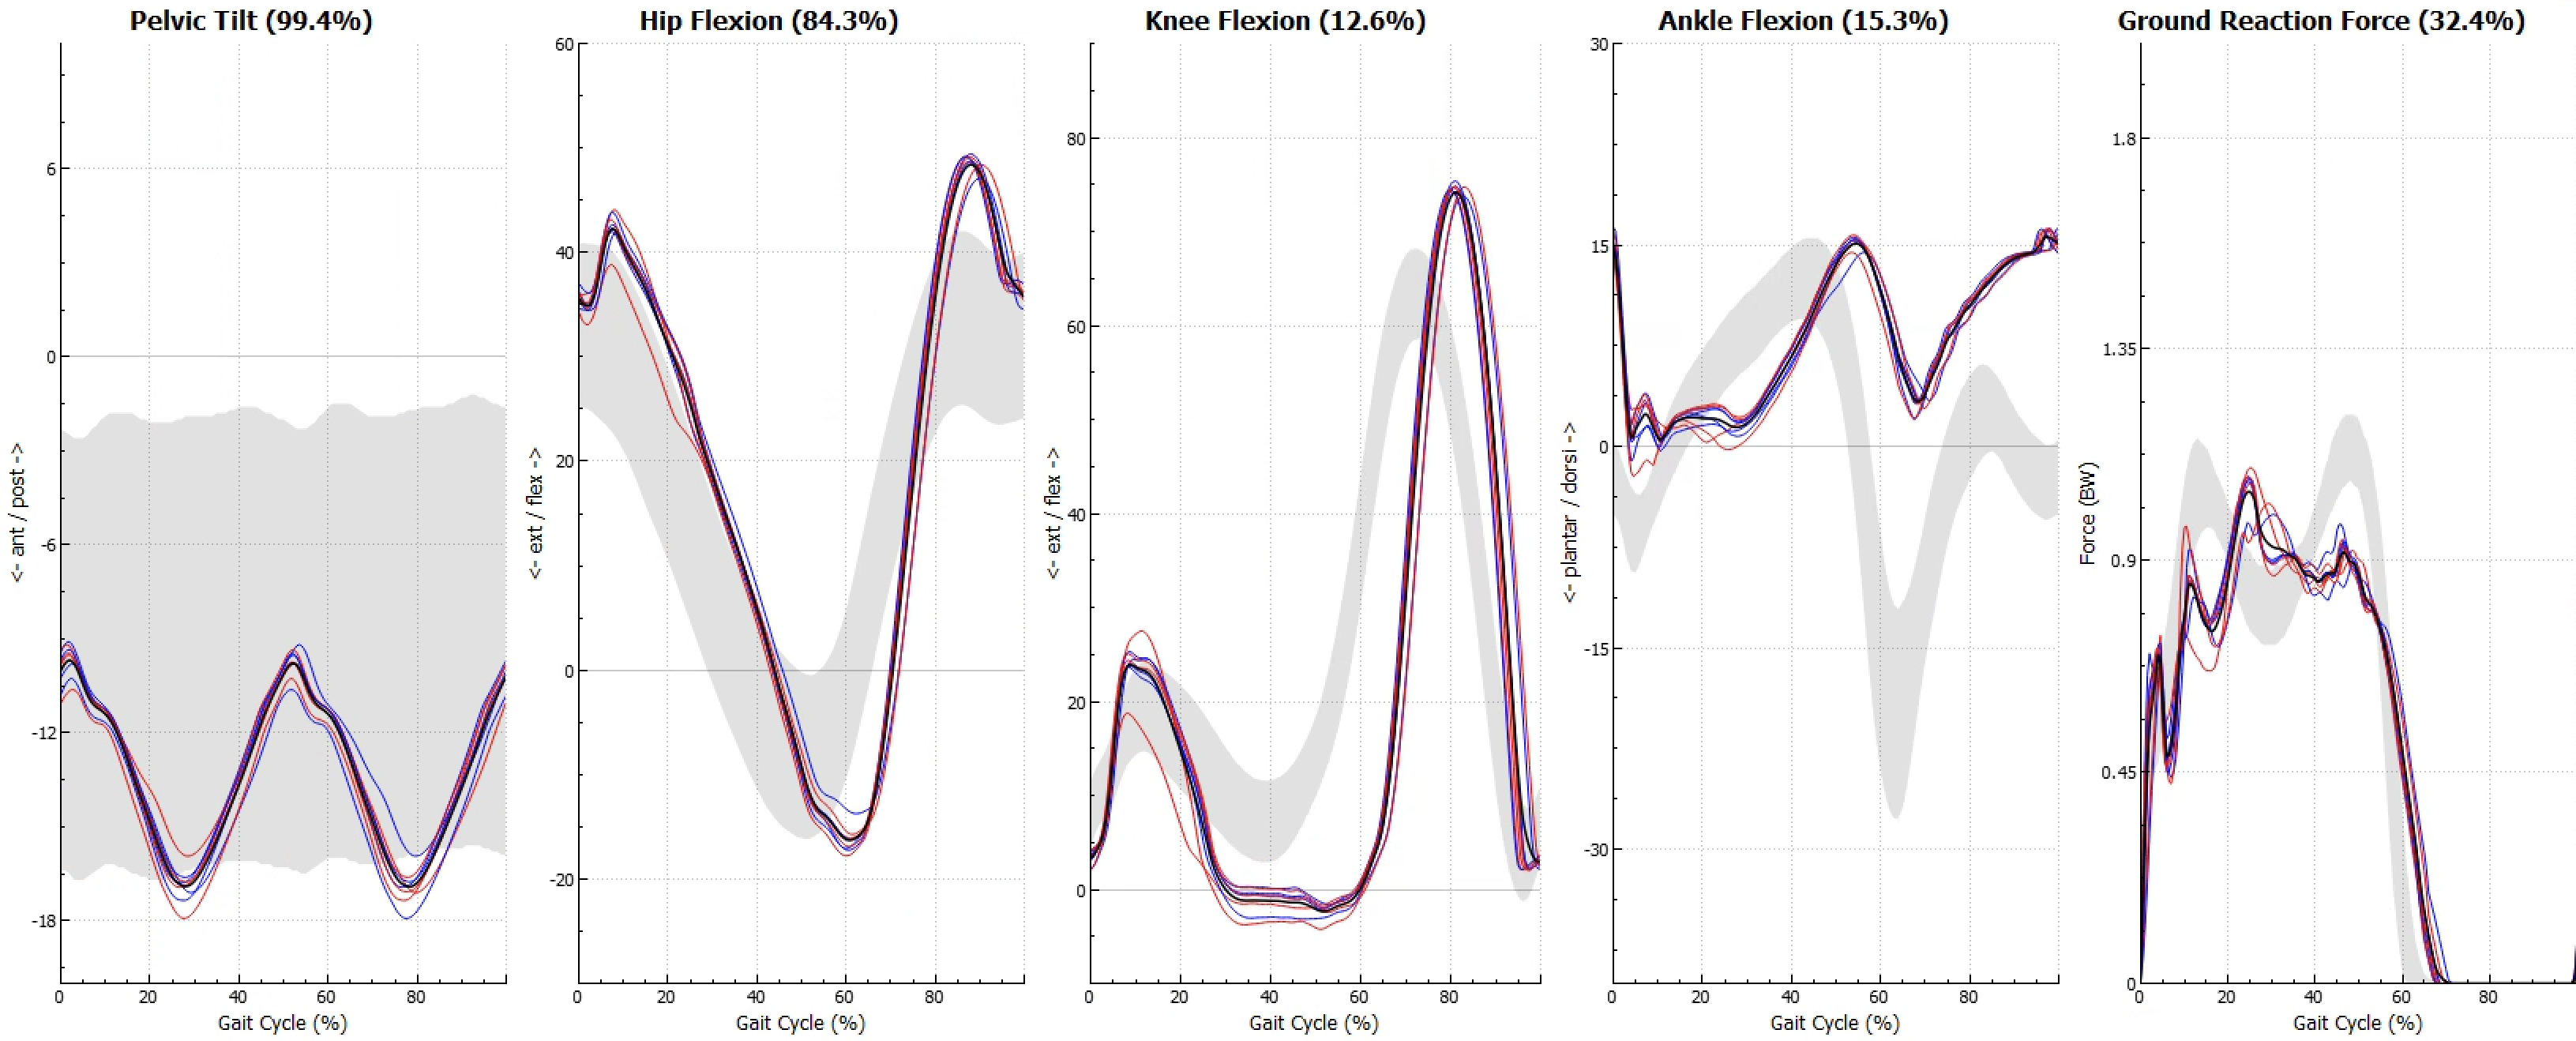
\includegraphics[width=\textwidth]{screens/atrophy_gait.png}
    \caption{Gait parameters as observed in the SCONE simulation of a subject with a gait affected by PF muscular atrophy.}
    \label{atrophic_gait}
\end{figure}

The resulting gait displays a \textit{heel-walking} behavior as is clearly visible on the rendering of figure \ref{atrophic_render}. As the body cannot produce any torque on the heel the lays flat on the ground for the entire support phase.

\begin{figure}[h!]
    \centering
    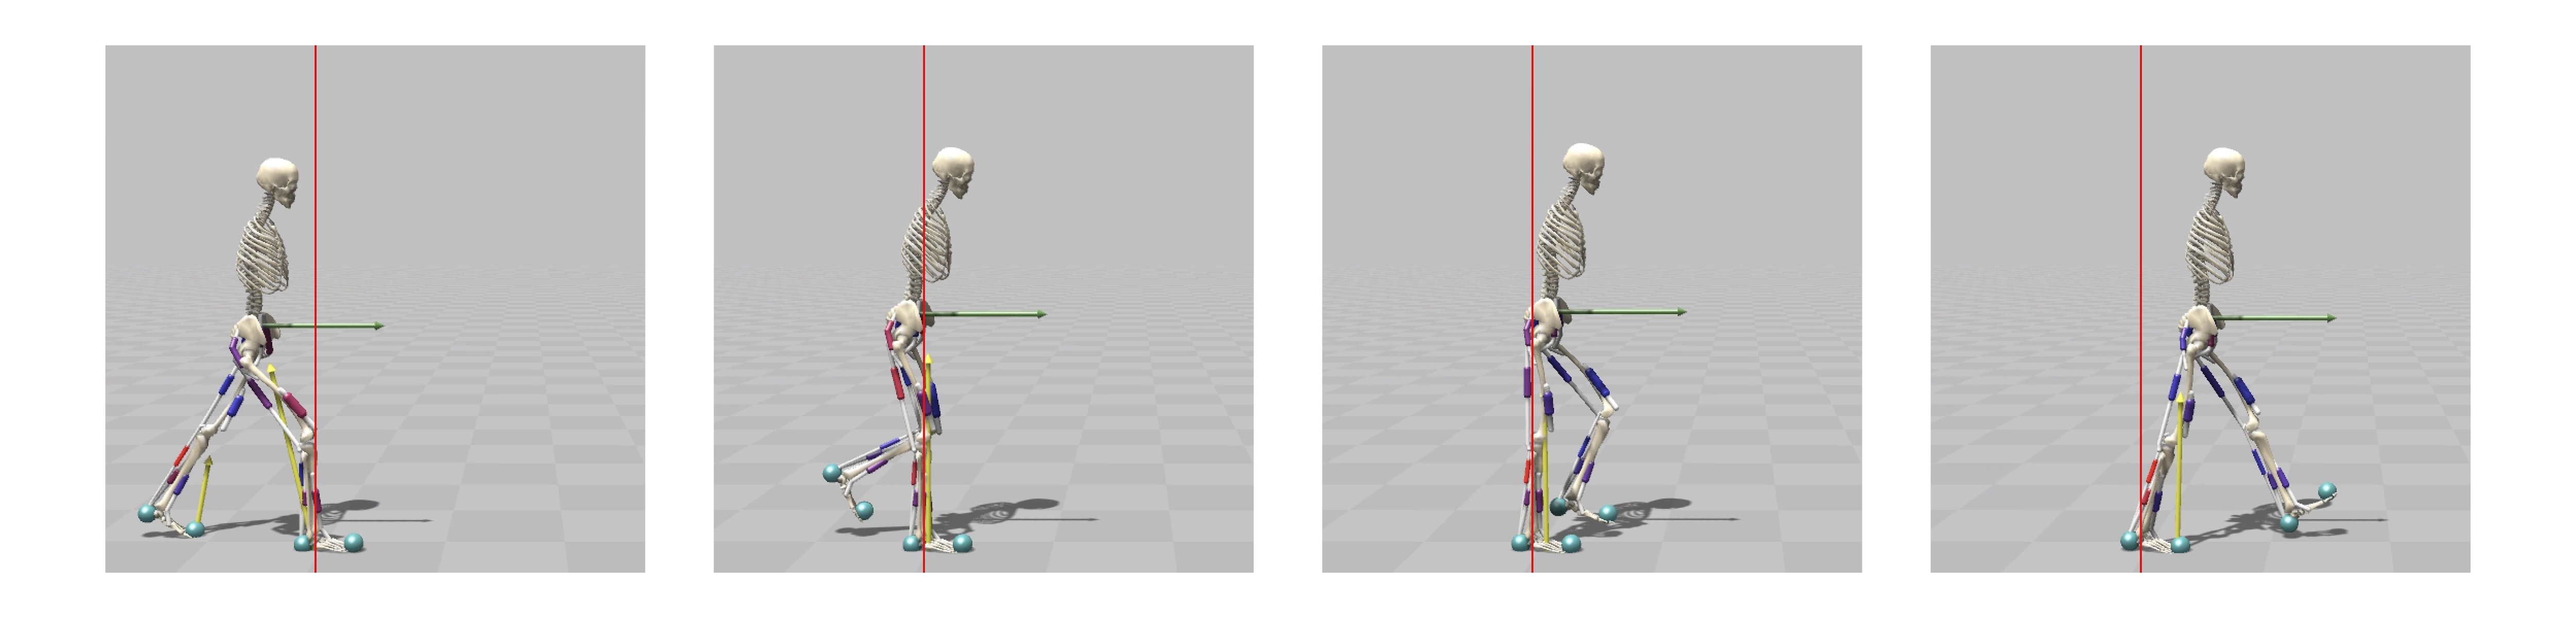
\includegraphics[width=\textwidth]{screens/heel_walk.jpg}
    \caption{Rendering of the optimization solution produced for the PF muscular atrophy model.}
    \label{atrophic_render}
\end{figure}

\section{Pathological Gait : Hyperreflexia}

We increase the gain of velocity dependent reflexes for both plantarflexor muscles in the model controller and run the optimization process until we find a stable gait. We clearly see that the principal kinematic adaptation is that the model adopts a \textit{toe-walking} gait. This can be observed in the ankle flexion plot  from the gait analysis (figure \ref{hr_gait}) which adopts a constant negative value (the heel is almost never flat on the ground) or in the renders (figure \ref{hr_render}) that clearly show that the body supports itself on the toe alone for the entire support phase. The knee flexion amplitude is also increased. The pelvic tilt also displays a higher average value than for both previous gaits (which actually makes it more in line with average, healthy human walking).

\begin{figure}[h!]
    \centering
    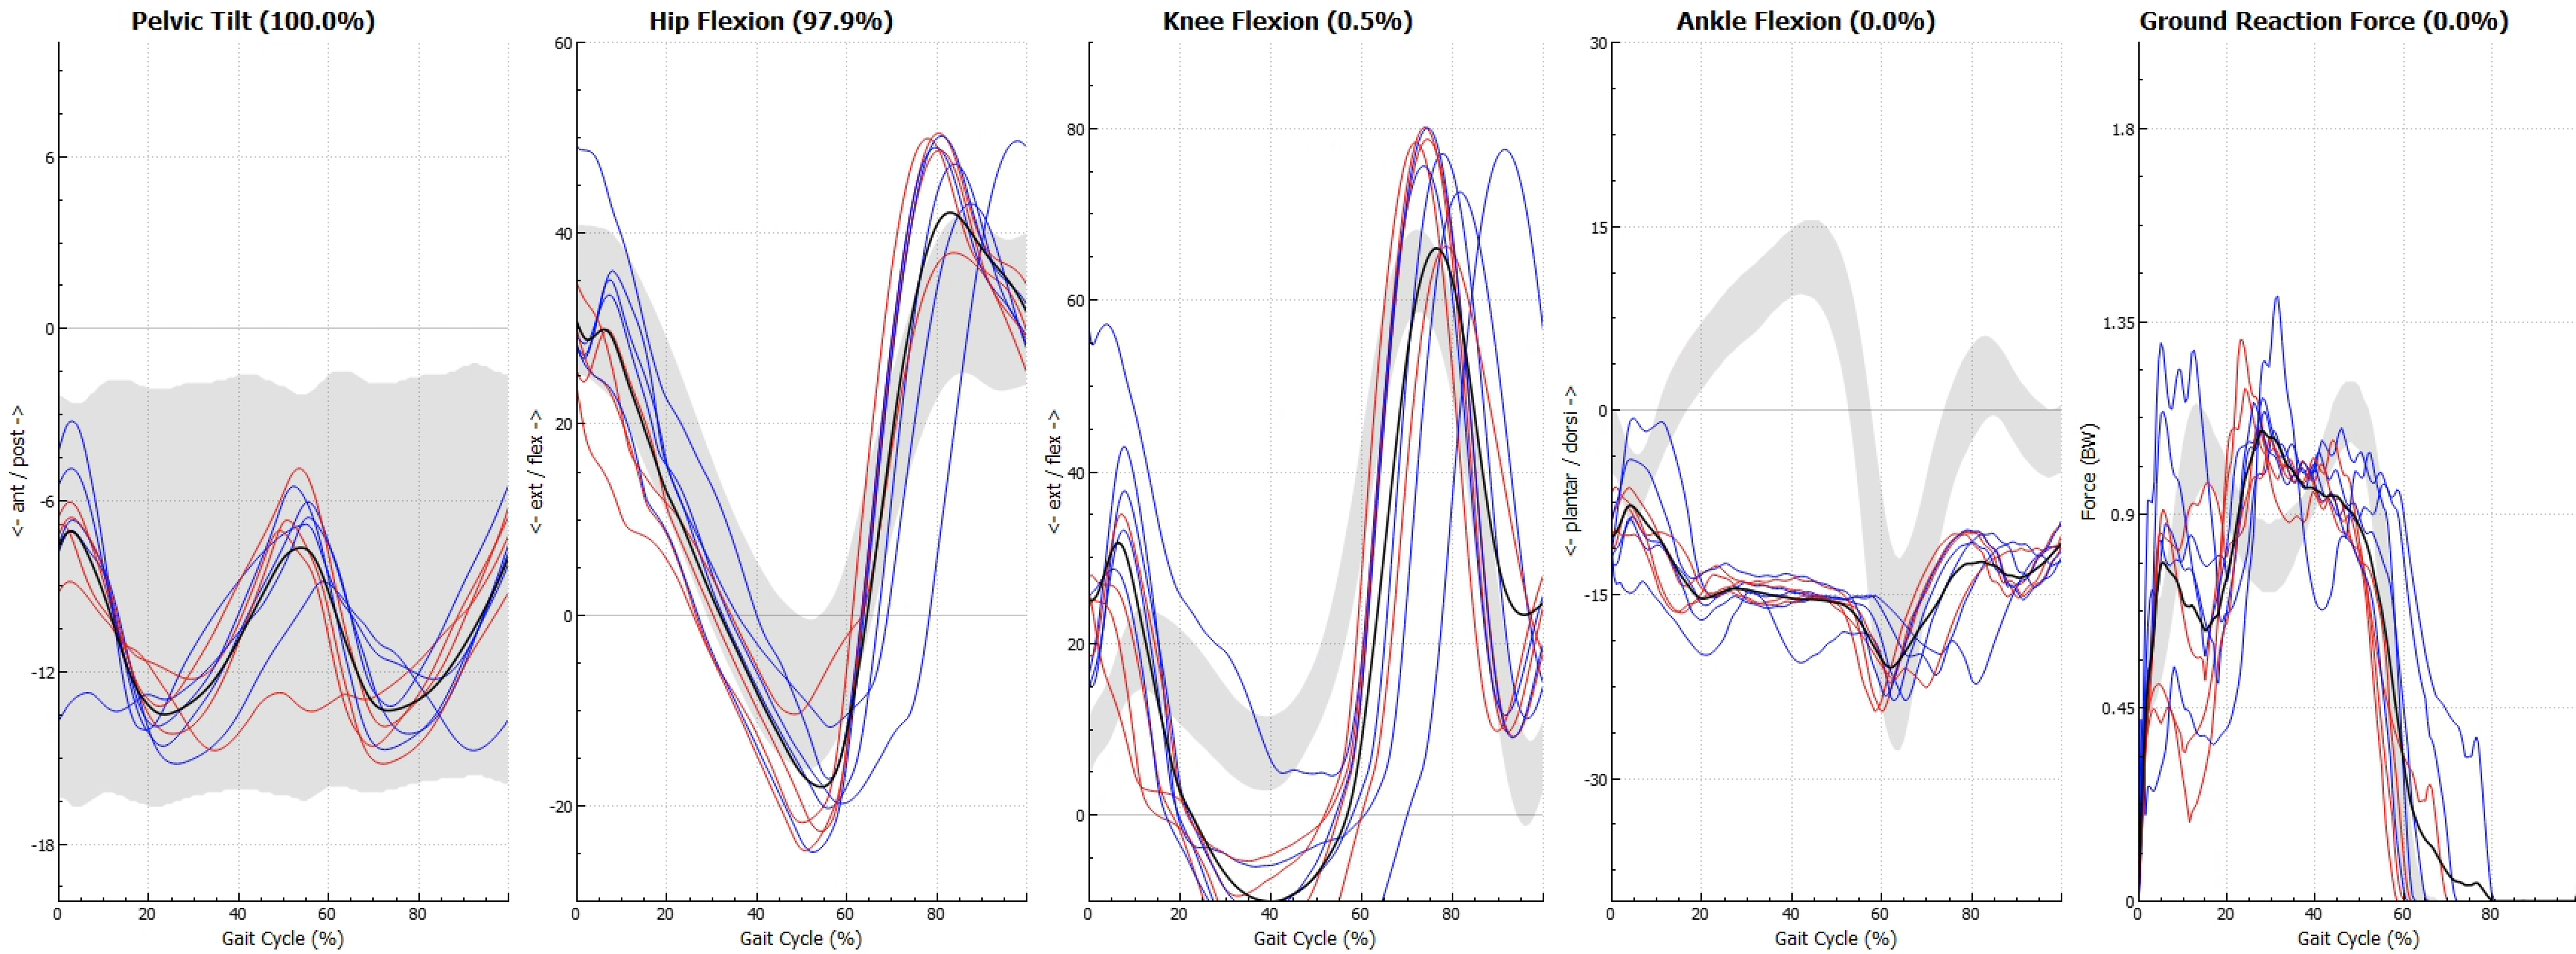
\includegraphics[width=\textwidth]{screens/hyperreflexia_gait.png}
    \caption{Gait parameters as observed in the SCONE simulation of a subject with a gait affected by hyperreflexia. We observe that the signal is more noisy, and has a higher amplitude on every variable. }
    \label{hr_gait}
\end{figure}

Furthermore we observe that the gait signal is significantly more noisy on all variables compared with both the healthy and muscle atrophic gait. From a control theory perspective it actually quite unsurprising that a stronger feedback leads to a higher instability in a closed loop dynamical system.

\begin{figure}[h!]
    \centering
    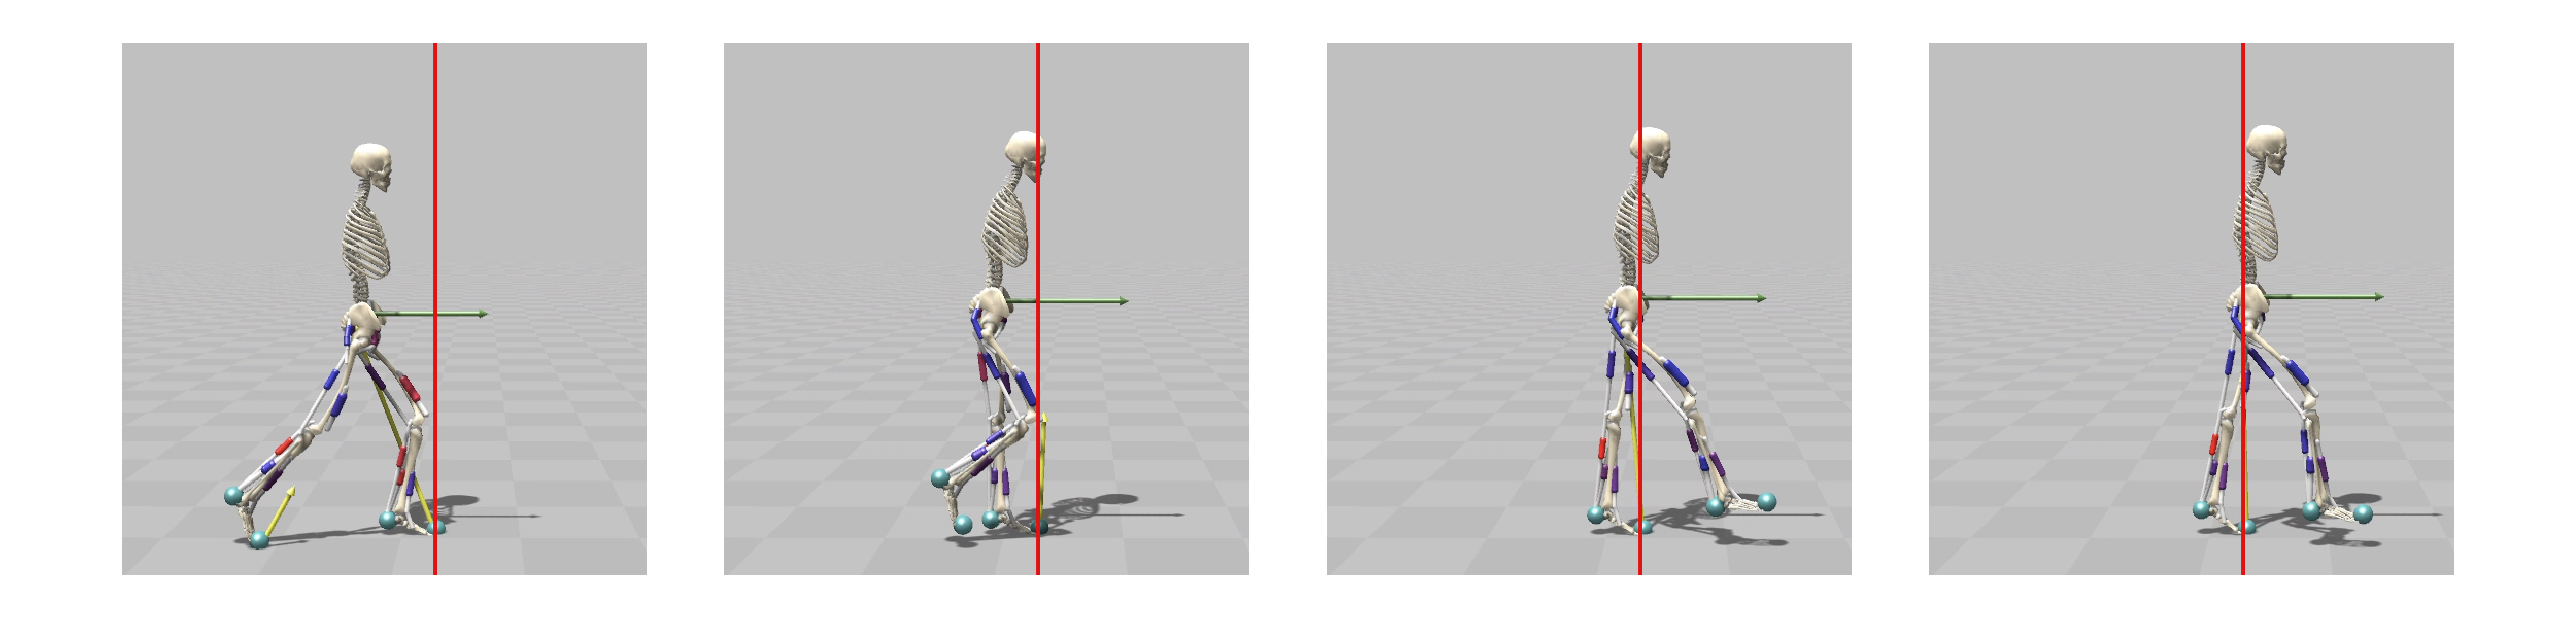
\includegraphics[width=\textwidth]{screens/toe_walk_hr.jpg}
    \caption{Rendering of the optimization solution produced for the hyperreflexia model.}
    \label{hr_render}
\end{figure}

\section{Pathological Gait : Toe Walking}

We try to reproduce a pathological gait that displays toe-walking. To get to such a gait we propose an alteration to the OpenSim model to emulate plantarflexor muscle contracture (as proposed by Ong et al. \cite{1}). We implement severe PF contracture by reducing the optimal fiber length of left and right \textit{soleus} an \textit{gastrocnemius} muscles by a factor of $0.7$. After running the optimization process we observe that the solution indeed converges to a toe-walking gait that is quite similar to the one observed when modeling hyperreflexia. The resulting gait is less noisy than the one obtained by modeling hyperreflexia (figure \ref{toe_gait}), but the gait is quite irregular (it differs from one cycle to another). The knee flexion amplitude is also lower than in the hyperreflexia example.

\begin{figure}[h!]
    \centering
    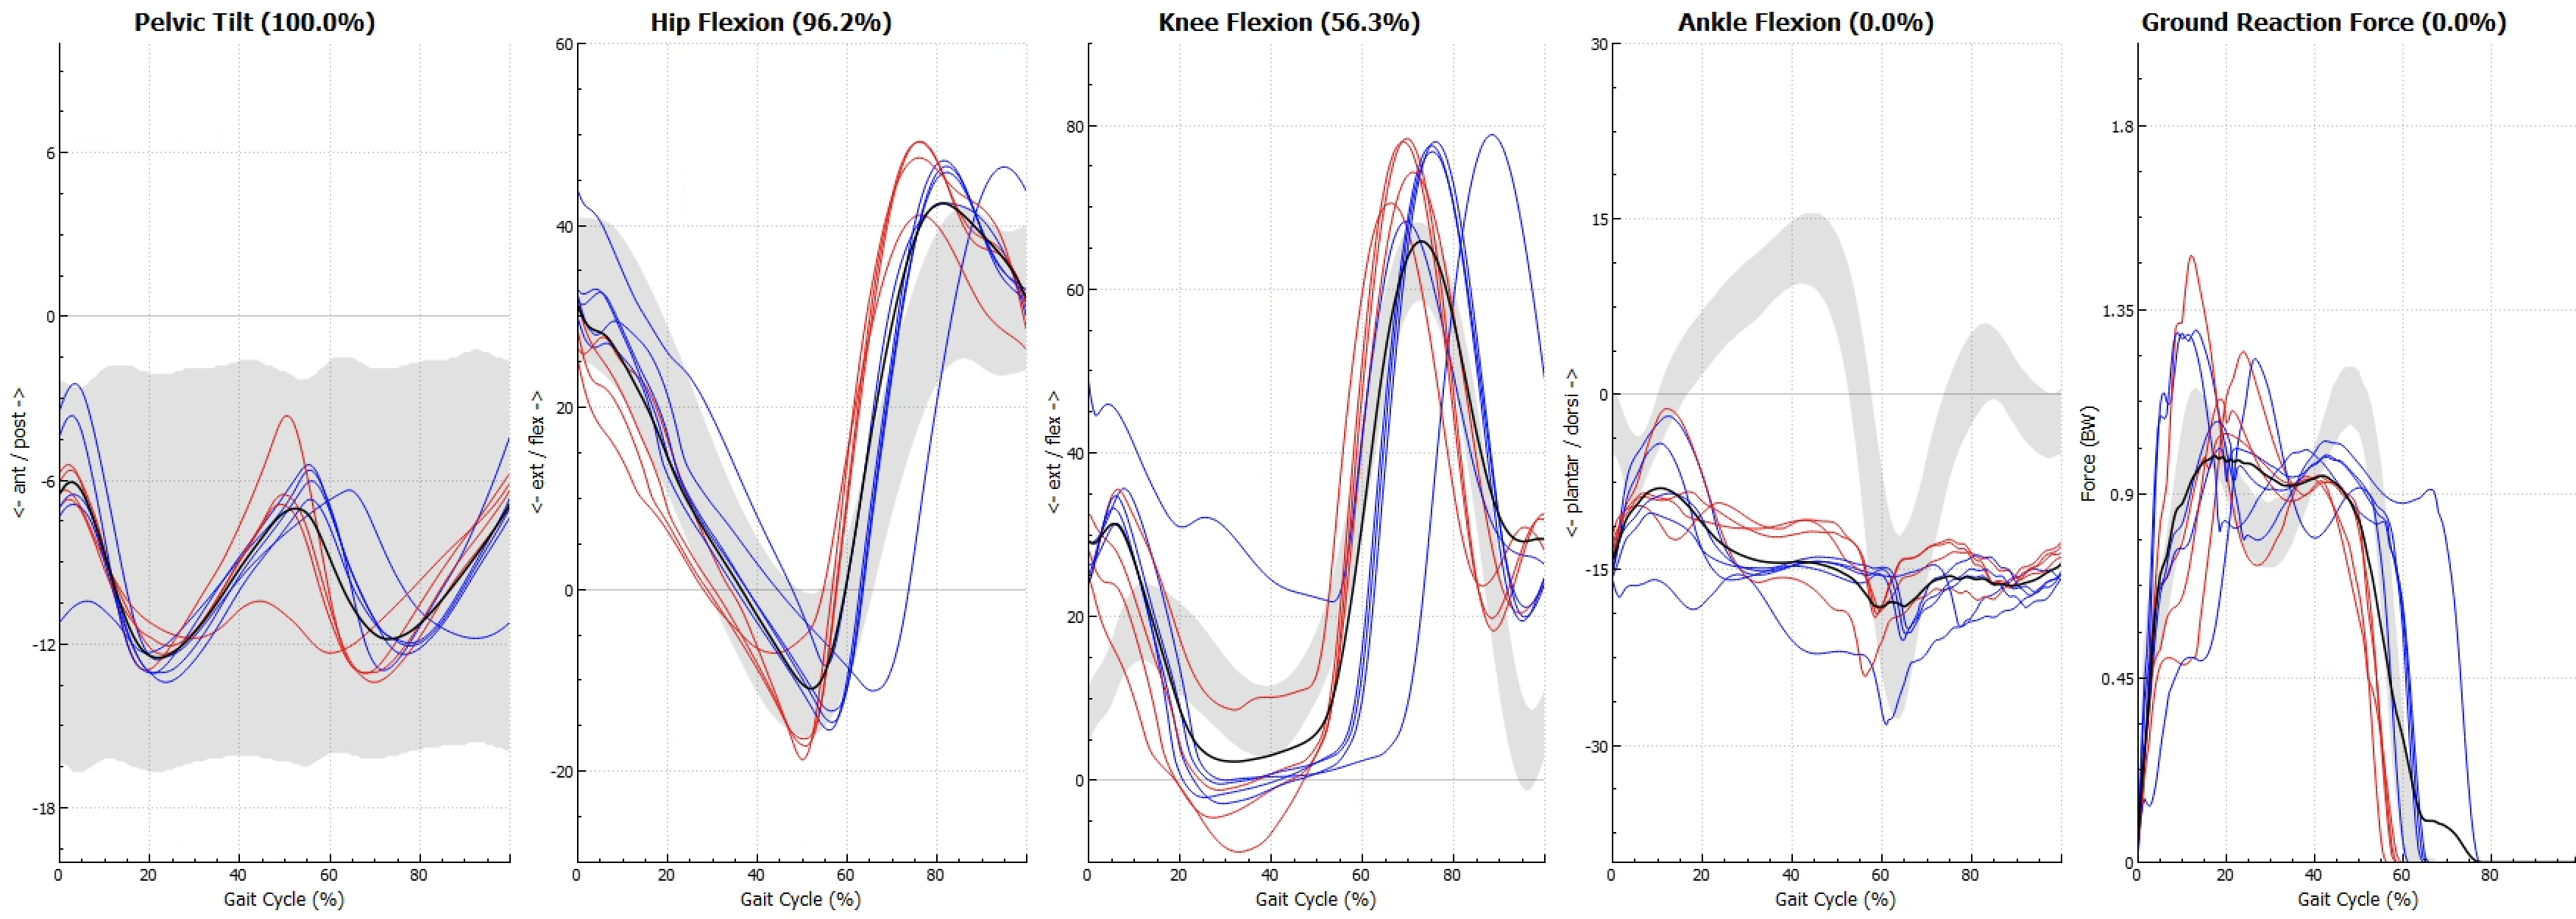
\includegraphics[width=\textwidth]{screens/toe_walk_gait.png}
    \caption{Gait parameters as observed in the SCONE simulation of a subject with a gait affected by severe PF contracture.}
    \label{toe_gait}
\end{figure}

\begin{figure}[h!]
    \centering
    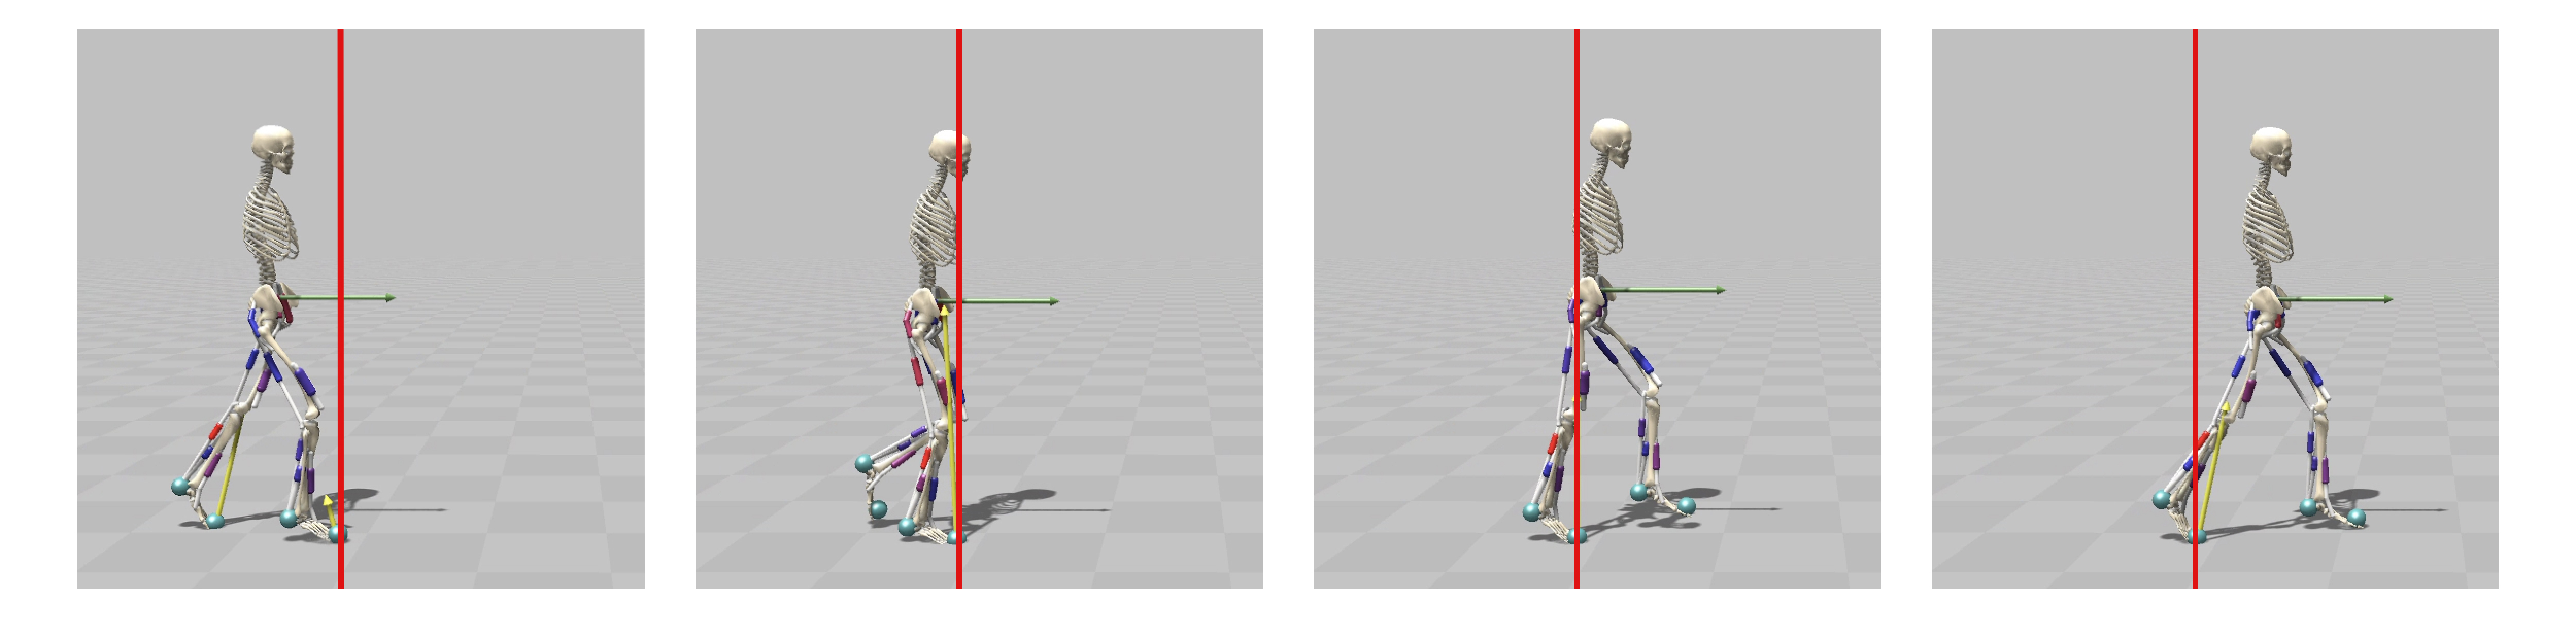
\includegraphics[width=\textwidth]{screens/toe_render.jpg}
    \caption{Rendering of the optimization solution produced for the toe-walking model (subject affected with severe PF contracture).}
    \label{toe_render}
\end{figure}


\begin{thebibliography}{1}

    \bibitem{Ong} Ong CF., Geijtenbeek T., Hicks JL., Delp SL., "\textit{Predicting gait adaptations due to ankle plantarflexor muscle weakness and contracture using physics-based musculoskeletal simulations}" \emph{PLoS Computational Biology 15}, 2019.
\end{thebibliography}


\end{document}

